% Chapter for alternative methods to solving the problem.

\chapter{Methods}

In this Section, I discuss my solution to the problem and various alternatives I
considered along the way.

\section{Overview}

I solved this problem by formulating it as a search problem. By this I mean,
given a schematic of a circuit, I start from an empty protoboard, and I search
through the space of all possible protoboard layouts to find the protoboard
corresponding to the schematic at hand. The space of all possible protoboards is
very large \q, so I utilize various simplifications
and heuristics to facilitate the search.

I broke down the problem into two parts. The first task is finding a placement
of all the circuit pieces on the protoboard. The second task is wiring them up
appropriately.

\section{Part 1: Piece Placement}

Let us first consider how to place a set of circuit pieces on the protoboard for
a given circuit schematic.

\subsection{The Pieces}

Any given circuit may contain resistors, Op Amps, pots, motors, head connector
parts, or robot connector parts. For each of these components, we must put down
a corresponding piece on the protoboard.

\subsubsection{Resistors}
\label{sec:resistor_pieces}

For the sake of simplicity, and to significantly reduce the search space
\q, for every resistor in the schematic, I use one
resistor piece on the protoboard placed in the middle strip of the protoboard
as shown in Figure \ref{fig:piece_placement}. This choice, i.e. allowing the
resistor pieces to only reside in the middle strip of the protoboard, is critical
as the resistor pieces can generally be placed at numerous places on the
protoboard.
With this restriction, there are $63$ slots available for one resistor. Without
this restriction, there are a total of $763$ slots available. The restirction is
good when we consider the reduction in the search space size. On the other hand,
the restriction is bad when we
consider the size of circuits the algorithm can layout. Given that the number
of resistors in a typical 6.01 circuit is very
small \q, this restriction proves
to be very useful, but we will consider the alternative in Section
\ref{sec:resistors_as_wires}.

\begin{figure}
\begin{center}
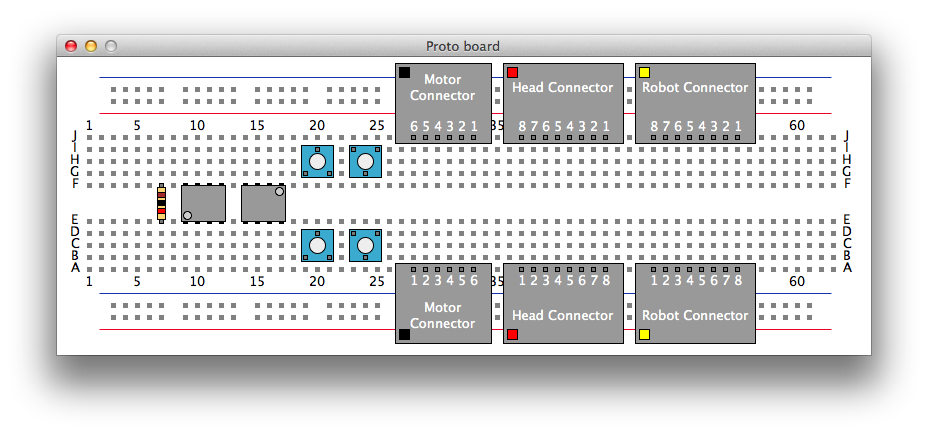
\includegraphics[width=\linewidth]{Images/piece_placement_options.png}
\caption{Various acceptable ways of putting each of the circuit pieces on the
protoboard.}
\label{fig:piece_placement}
\end{center}
\end{figure}

\subsubsection{Op Amps}

Op Amps are the trickiest components to handle because each Op Amp package put
on the protoboard contains two Op Amps within it. Thus, we face the task of
packaging the Op Amps in the schematic in the ``best" possible way, i.e. so as
to require as little work as possible when wiring the pieces together. Equation
\ref{eq:opamp} presents an expression for the value $f(n)$, the number of
different ways to package together $n$ Op Amps. For example, if we have $2$ Op
Amps, we can either use one Op Amp package for each, or put them both in the
same package, which we can do in one of two different ways. Hence, $f(2) = 3$.
To get a sense of how many different packagings are possible, Table
\ref{tb:opamp} gives the values of $f(n)$ for various $n$.

\begin{equation}
f(n) = \sum\limits_{k=0}^{\lfloor\frac{n}{2}\rfloor}{\frac{n!}{k!(n - 2k)!}}
\label{eq:opamp}
\end{equation}

\begin{table}
\begin{center}
\begin{singlespace}
\begin{tabular}{c | c}
$n$ & $f(n)$ \\
\hline
\hline
1 & 1 \\
2 & 3 \\
3 & 7 \\
4 & 25 \\
5 & 81 \\
6 & 331 \\
7 & 1303 \\
8 & 5937 \\
9 & 26785 \\
10 & 133651
\end{tabular}
\end{singlespace}
\end{center}
\label{tb:opamp}
\caption{Number of ways of packaging together $n$ Op Amps for various values of
$n$.}
\end{table}

Each Op Amp package is placed in the middle strip of the protoboard, with two
acceptable orientations, as shown in Figure \ref{fig:piece_placement}.

\subsubsection{Pots}

Each pot piece can be placed in one of two vertical locations on the protoboard.
Each pot piece also has two possible orientations. Figure
\ref{fig:piece_placement} provides examples of all acceptable options.

\subsubsection{Head, Motor, and Robot Connectors}

We use a 6-pin connector to connect to a motor, and an 8-pin connector to
connect to either a head or a robot. Each connector can be placed in one of two
vertical locations on the protoboard, as shown in Figure
\ref{fig:piece_placement}.

\subsection{Choosing a Placement}

When choosing a placement of circuit pieces on the protoboard, we have at hand a
plethora of options. First we must choose among a possibly large number of ways
to package together the Op Amps in the circuit. For each possible packaging of
Op Amps, we must consider various ways of placing the pieces on the protoboard.

\subsubsection{Simplifications}

I reduce this large number of options by only allowing placements in which no
two pieces share a column. Once again, this is not necessary in general, but the
number of pieces necessary for a typical 6.01 circuit would certainly fit in
this framework.

Next, I specify that there be exactly two columns on the protoboard separating
each consecuitive pair of pieces, unless the pieces are both resistors, in which
case there must be exactly one column separating them. These numbers of columns
were chosen to leave enough space for wiring. Given a set of pieces to be put on
the protoboard, this specification reduces the
problem of choosing a placement for the pieces to finding an \emph{order} of the
pieces together with choosing their respective vertical locations and
orientations.

Given these simplifications, we have various options as to how to pick a
placement.

\subsubsection{Random Placement}

One simple alternative may be to choose a placement randomly. That is, we choose
an Op Amp packaging randomly; we choose an order of the pieces randomly; and we
choose the vertical locations and orientations of the pieces randomly as well.
The advantage of this
approach is that it gives us a placement very quickly without requiring much
computation. On the other hand, we may end up placing two pieces that need to be
connected to each other very far apart, and we will have a difficult time doing
the wiring. Hence, we ought to consider alternatives in which we take into
account the task of wiring. We should try to place the pieces so as to require
as little work during wiring as possible.

\subsubsection{Minimal Heuristic Cost}

The key idea is that if two pieces are meant to be connected together by wires,
then they ought to be placed close to each other on the protoboard. We can
capture this idea by assigning heuristic costs to the placements and choosing
a placement that produces the minimal heuristic cost.

Let us first devise the cost function to achieve this goal. Given a circuit
schematic and a corresponding placement of the circuit pieces on the protoboard,
what do we need to connect with wires? Well, every pair of components in the
schematic that are connected by a wire gives us a corresponding pair of
locations on the protoboard that ought to be connected by wires. However, we can
express this requirement a little bit more concisely. We ought to consider all
of the nodes in the schematic, and find the circuit components in the schematic
that are connected to the respective nodes. Now for each node in the circuit, we
get a set of locations on the protoboard that ought to be interconnected. The
first step in devising the cost function we are looking for is to have a way to
estimate the cost of connecting two locations on the protoboard. A simple such
cost function that comes to mind is the Manhattan distance between the two
locations. Recall that we want to produce aesthetically pleasing protoboard
layouts, and one of the requirements in achieving this goal is only using
horizontal and vertical wires (i.e. no diagonal wires) so the Manhattan distance
cost is appropriate. Given this heuristic cost for connecting two locations with
wires, we can define the heuristic cost for interconnecting the locations
associated with a particular node to be the weight of the minimum spanning tree
of the locations. Now we can define the cost of a placement to be the sum over
all nodes in the circuit of the cost for interconnecting the locations for each
node.

Now that we have a cost function for placements, we can aim to find a
placement with the minimal cost. However, this involves trying all possible
orderings of the pieces with which we are working. For example, if we are trying
to order $10$ pieces, we would need to look at $10! = 3628800$ possible
orderings \q. Note that this is in addition to
searching over all possible ways
of packaging the Op Amps together. It is clear to see that the search for a
minimal cost placement quickly gets out of hand. So we aim to find a placement
that has a very small, though maybe not minimal, cost.

\subsubsection{Small Heuristic Cost}

Algorithm \ref{alg:small_cost_placement} presents a polynomial-time procedure
that orders a
given list of pieces in a way that results in a small cost. The algorithm places
one of the pieces at a time, starting from an empty placement. It relies
on two ideas. First, once a piece has been placed, all the pieces that are
connected to it will be placed soon after so that it is more likely that those
pieces are placed close to it. Second, we place the pieces with the most nodes
first since those are the ones that most likely have connections with many other
pieces.

\begin{algorithm}
\KwData{A list $P$ of circuit pieces.}
\KwResult{A list $R$ of circuit pieces representing a placement.}
\BlankLine
Sort $P$ in decreasing number of nodes on the respective pieces\\
$Q$ $\leftarrow$ empty Queue\\
$R$ $\leftarrow$ empty List\\
\While{$P$ is not empty}{
Pop the first piece in $P$ and push it onto $Q$\\
\While{$Q$ is not empty}{
$p$ $\leftarrow$ $Q$.pop()\\
Consider all vertical locations and orientations of $p$\\
Place $p$ at an index in $R$ that minimizes the cost of $P$\\
\ForEach{piece $q$ in $P$ connected to $p$}{
Pop $q$ out of $P$ and push it onto $Q$\\
}}}
\caption{Producing a circuit piece placement with small heuristic cost.}
\label{alg:small_cost_placement}
\end{algorithm}

Using one of the above methods, we can find a placement of circuit pieces on a
protoboard. Our next task is wiring them together to produce a circuit
equivalent to the circuit schematic of interest.

\section{Part 2: Wiring}

In the previous section we discussed what locations we need to wire together:
for every node in the circuit, we get a set of locations on the protoboard that
need to be interconnected. The question now is how to achieve this wiring. We
approach the problem as a search problem and use the $A*$ search algorithm to
solve it.

\subsection{Using $A*$}

When using the $A*$ algorithm, we need to design four things:

\begin{enumerate}
\item The notion of a vertex\footnote{The prefered name is ``node" but I will
use vertex since we already use node to refer to nodes in circuits.} in the
search tree, the cost associated with a vertex, and how we obtain the neighbors
of a vertex,
\item The starting vertex,
\item How we identify whether a particular vertex in the search tree achieves
the goal of the search, and
\item A heuristic function that estimates the distance from a given vertex to a
goal vertex.
\end{enumerate}

\subsection{Vertices}

Each vertex will hold a representation of some protoboard. Each representation
will contain all of the pieces, and possibly a set of wires interconnecting the
pieces. The starting vertex will have all of the pieces but no wires.

We obtain the neighbors of a vertex by taking the current protoboard and
producing new ones in which we place exactly one wire at various locations. We
choose the starting point of a wire to be any one of the free locations on the
protoboard that is already connected to one of the pieces, and we extend the
wires in all possible vertical and horizontal directions up to some fixed wire
length. Note that we need
to take great care when placing wires in order not to short different nodes. We
discard any vertices that arise from placing a wire that shorts two different
nodes.

The way we define the cost of a vertex, i.e. the cost of getting from the
starting vertex to a vertex of interest, depends on what we consider to be an
aesthetically pleasing protoboard layout. In general, we want to penalize having
long wires, many wires, or crossing wires. In my implementation, while I have
a large penalty for two crossing wires of opposite orientations (i.e. vertical
and horizontal), I do not allow crossing wires that have the same orientation as
this configuration is particularly difficult to physically build and debug.
Finally, we want to favor making a desired interconnection between locations
on the protoboard. I chose my penalties experimentally
\q.

Each vertex will not only hold a protoboard, but it will also hold a set of
pairs of locations on the protoboard that need to be connected by wires. Each
pair $(loc_1, loc_2)$ of locations tells us that we need to have a set of wires
connecting some location connected to $loc_1$ to some location connected to
$loc_2$.

An important consideration we need to make is how we want to organize the
search. Recall that we have a set of nodes in the circuit of interest, and for
each node we have a set of locations that need to be interconnected. Given this
information, we may choose one of the following three strategies to carryout the
search:

\begin{enumerate}
\item For each node, collect a set of pairs of locations on the protoboard
corresponding to a minimum spanning tree of the locations for that node, so that
if all pairs of locations in this spanning tree are connected, then the
locations for the node will be interconnected. Collect all such pairs of
locations for all of the nodes in the circuit, and have the starting vertex hold
this set of pairs of locations.
\item Treat each node separately. That is, iteratively interconnect the
locations for each of the nodes until there are no more nodes in the circuit.
\item Treat each pair of locations that needs to be connected separately. That
is, iteratively connect pairs of locations that need to be connected until there
are no more pairs.
\end{enumerate}

The choice of one of these strategies has a significant effect on the outcome of
the search. We will discuss the difference in detail in Chapter
\ref{ch:results}.

\subsection{Goal test}

Given a vertex, we know that it is a goal vertex if all of the pairs of
locations it holds are already connected in the protoboard it holds.

\subsection{Search heuristic}

In $A*$ search, choosing the right heuristic can often make the search much more
efficient. In our problem, one option we have is not to use a heuristic, and
that alternative will be explored in Chapter \ref{ch:results}. However there is
a natural heuristic that suggests itself that we ought to consider. Given a
vertex, we can estimate its distance from a goal as follows. For each pair of
locations $(loc_1, loc_2)$ that need to be connected, we could consider its
distance from the
goal to be the smallest Manhattan distance between any location connected to
$loc_1$ and any other location connected to $loc_2$. To compute the heuristic
cost of a vertex, we simply add up this value for each of the pairs of locations
that need to be connected. Chapter \ref{ch:results} presents the performance of
this heuristic verses using no heuristic.

\section{Treating Resistors as Wires}
\label{sec:resistors_as_wires}

The discussion in Section \ref{sec:resistor_pieces} presented that we treat
resistors just as we do the other components. That is, we give each resistor a
fixed place on the protoboard in the first step of the algorithm before the
wiring step. However, resistors have the special property among the circuit
pieces that they can be thought of as wires of length $3$.
Hence, it may be possible to handle resistors in the wiring step instead of the
placement step. Chapter \ref{ch:results} presents a comparison of these two
approaches.

Note that treating resistors in the wiring step is not a trivial task. First,
there may be nodes in the circuit that are connected to some resistors, but no
other pieces. In this case, we must be sure to reserve space on the protoboard
for that node as the wiring step relies on the presence of each node on the
protoboard. Second, we must keep careful track of pairs of locations that need
to be connected by simple wires and pairs of locations that need to be connected
using resistors.

\label{sec:resistors_as_wires}
